%%%%%%%%%%%%%%%%%%%%%%%%%%%%%%%%%%%%%%%%%%%%%%%%%%%%%%%%%%%%%%%%%%%%%%%%
\chapter{Background}
\label{ch:background}
%%%%%%%%%%%%%%%%%%%%%%%%%%%%%%%%%%%%%%%%%%%%%%%%%%%%%%%%%%%%%%%%%%%%%%%%

Machine Learning popularity exploded in last years. If you work in tech
it is hard you did not hear about large public datasets, neural
networks, deep learning, or just how people speculate a majority of
jobs will be substitued by machine trained from data.

Apart from a noisy hype, many services are actually built using Machine
Learning and implementing them using different techniques is nearly
impossible. Think of how Spotify generates playlists that are tailored
to you musical
taste\footnote{https://support.spotify.com/us/article/daily-mix/}, or
just how YouTube gives you suggestions specifically for you
\cite{45530} --- even when you should do more serious
work\footnote{``Why quitting smartphones is the new quitting smoking'' https://www.ft.com/content/4f82a008-0096-11e8-9650-9c0ad2d7c5b5}.

More and more developers are getting interested in this kind of
technology and as more people work on these topics, more people build
better tools, empoweing larger groups of developers to write
services using Machine Learning.

This chapter is organized as follows: Section
\ref{sec:machine-learning} is about what is Machine Learning and the
gradient descent procedure; in Section \ref{sec:neural-networks} we will
describe Neural Networks, a classifier that is used with great success
in recent times; Section \ref{sec:adversarial-examples} explains what
are adversarial examples and how they are generated.

\section{Machine Learning}
\label{sec:machine-learning}

Quoting
Wikipedia\footnote{https://en.wikipedia.org/wiki/Machine\_learning}

\begin{quote}
Machine learning is a field of computer science that uses statistical
techniques to give computer systems the ability to "learn" (e.g.,
progressively improve performance on a specific task) with data,
without being explicitly programmed.
\end{quote}

\begin{figure}
  \centering
  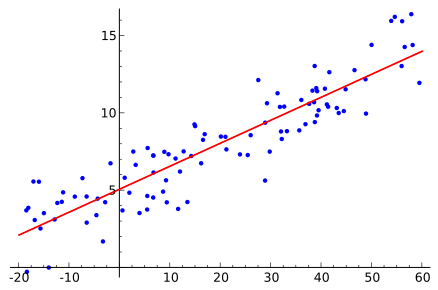
\includegraphics[width=0.5\linewidth]{Images/wikipedia-linear-regression.png}
  \caption{A linear model built out of a dataset. By Sewaqu [Public
      domain], from Wikimedia Commons}
  \label{fig:wikipedia-linear-regression}
\end{figure}

A typical example to introduce people with some scientific preparation
to this topic is the one of linear regression \cite{B071JXYDDB}. In
linear regression you have data coming in pairs $(x, y)$ and you think
that $y$ can be linearly dependent on $x$. That is, your hypothesis is

\begin{equation}
  y = w x + b
  \label{eq:linear-model}
\end{equation}

where $w$ and $b$ are called the weight and the bias
respectively\footnote{In other fields, $w$ and $b$ are more commonly
  known as the slope and the intercept.}. The problem is to find the
best values $w^*$ and $b^*$ such that $y^*$ defined as

\[ y^* = w^* x + b^* \]

is the closest possible to the associated value of $y$.

When both $x$ and $y$ are scalar, the problem of finding the best
values $w^*$ and $b^*$ becomes the problem of finding the best line
that is the \emph{closest} to all the data --- see Figure
\ref{fig:wikipedia-linear-regression}.

In general there are no \emph{correct} values for $w^*$ and
$b^*$ so you either estimate them using analytical methods like the ones
you probably learned in some math course or you derive the two values
using a data-based procedure that minimizes the
distance between the expected and the actual value of $y$.

The function that computes the distance is generally called the
\emph{loss} function and can be as simple as the $L_1$ distance
\cite{taxicab-geometry} --- i.e. the absolute value of the difference
of the two values. Instead the algorithm that minimizes the loss can be
any minimization procedure; one of the most known one is called the
gradient descent \cite{Goodfellow-et-al-2016}. The gradient descent
procedure to minimize a general function $F(\boldsymbol{z}):
\mathbb{R}^n \rightarrow \mathbb{R}$ constists of iteratively computing

\begin{equation}
  \boldsymbol{z}_{n+1} = \boldsymbol{z}_n - \gamma
  \nabla{F}(\boldsymbol{z}_n)
\end{equation}

where $\boldsymbol{z}_n$ is the function argument at the algorithm's
nth iteration, $\gamma$ is the so-called \emph{learning rate} while
$\nabla{F}(\boldsymbol{z}_n)$ is the gradient of the loss function $F$
evaluated at $\boldsymbol{z}_n$. The idea behind the procedure is that
the gradient --- that when your model is a line collapses to just
being the derivative --- is used to find the \emph{direction} in which
the function is growing; then the procedure does an iterative step (whose size
depends on the learning rate $\gamma$) in the \emph{opposite}
direction. That is, the procedure identifies where the loss functions
is growing to perform a step towards a minimum instead. The minimum is
of course local --- it depends on where the procedure starts --- and
there is no guarantee that the algorithm will succeed in finding the
best of these minima.

This algorithm has nothing to do specifically with linear regression.
It is a general minimization algorithm. In fact, later in the thesis
we will use it even if we will never touch the topic of linear regression
again.

\section{Neural Networks}
\label{sec:neural-networks}

\begin{figure}
  \centering
  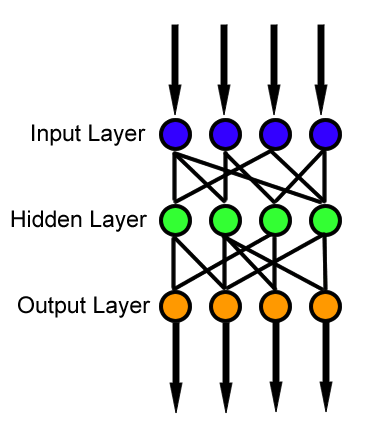
\includegraphics[width=0.5\linewidth]{Images/wikipedia-neural-network.png}
  \caption{Neural network example. By User:Paskari [Public domain], via
    Wikimedia Commons}
  \label{fig:wikipedia-neural-network}
\end{figure}

A neural network is one of the many models studied in Machine Learning.
There are a variety of neural network types, but the ones we used
throughout the thesis are called feedforward neural
networks \cite{Goodfellow-et-al-2016}.

A feedforward neural networks is one of the simpler neural networks and
it is the one that most people are first exposed to. Such a network is
organized as a stack of layers of neurons. A layer is just a sequence
of independent neurons, while a neuron is a \emph{computational unit}
that given an input and a state computes an output value.

In a feedforward neural network you have at least two layers: the input
layer and the output layer. The input layer has as many neurons as the
dimensions of the input --- e.g. if the input space is $\mathbb{R}^4$
the input layer will have four input neurons. Neurons in the input
layer do nothing but provide the other layers the data to make
computation on --- i.e. they all implements the identity function.
In the output layers we have as many neurons as the number of
classes in the classification task: each one has a value between 0 and
1, representing the confidence that the input belongs to that class.
For example, if the third neuron outputs a value of 0.577, according to
the model the current input belongs to the third class (the class
related to the third neuron) with a confidence of 57.7\%.

In between the input and output layer, you typically have one or more
the so-called \emph{hidden} layers. Each hidden layer (as the output
layer too) computes the composition of a linear function followed by
the application of a \emph{non}-linear function, called the activation
function. That is, each neuron computes

\[ \text{activation}(l \, W + b) \]

where $l$ is the state of the previous layer, while $W$ and $b$
represents the state of the neuron that changes as the model is
trained. The activation function can be any non-linear function; one of
the simplest one is called the rectifier

\[ \text{f}(z) = \text{max}(0, z) \]

This sequence of linear function and activation function can be
\emph{repeated} multiple times increasing the hidden layers of neurons.
Having several hidden layers of different width can improve the
performance of the model. When the network consists of many layers, the
network is referred to be a \emph{deep} neural network. As a rule of
thumb, the more the layers the better the performance of the model.
Yet, that is not always the case \emph{and} the deeper the network, the
longer it takes to train that model.

In fact, deep learning is not a new idea and many consider the recent
interest in neural networks as a consequence of the current available
computational power that was not there in the 20th century.

\begin{quote}
  Advances in hardware enabled the renewed interest. In 2009, Nvidia
  was involved in what was called the ``big bang'' of deep learning
  [...] [Andrew] Ng determined that GPUs could increase the speed of
  deep-learning systems by about 100 times. In particular, GPUs are
  well-suited for the matrix/vector math involved in machine learning.
  GPUs speed up training algorithms by orders of magnitude, reducing
  running times from weeks to days. Specialized hardware and algorithm
  optimizations can be used for efficient
  processing.\footnote{https://en.wikipedia.org/wiki/Deep\_learning\#History}
\end{quote}

The way we used neural networks has been for classification tasks, that
is given an input and a set of classes we want the network to be able
to assign that input to the correct class.

To understand how neural networks are used to perform classification it
is useful to know the concept of one-hot encoding of data. In one-hot
encoding possible values are binary numbers, that are legal only if
there is only one 1 --- e.g. 0001, 1000, ... but not 1001 or 1100.

One-hot encoding is used to map classes
in the training set to \emph{states} of the output neurons in the
neural network. For example, if the classification problem uses three
classes --- cat, dog and mockingbird --- a one-hot value will be assigned to
each class such to fit the \emph{shape} of the output layer --- that
is, it will be assigned 100 to the class of cats, 010 to dogs and 001
to mockingbirds.

During the training phase the network is \emph{shown} a
configuration of the input neurons (the single input example) and a
configuration of the output neurons (the class of the input example
one-hot encoded), and the network is \emph{confronted} with the
configuration of the output it obtains using its current weights and biases
in the hidden layers and \emph{tries} to reduce this distance. Of
course, it is the gradient descent procedure that does the job: the
network is actually a \emph{passive} object.

\section{Adversarial examples}
\label{sec:adversarial-examples}

Just like gradient descent is used to change the weights and biases of
the network to reduce the distance from the one-hot encoded class and
the actual output of the network, we can use gradient descent on the
input data to reduce the distance from the current output of the network to
another output of our choice. This way we can manipulate classification.

What we get is an input data generated from the original input but
modified in such a way that the input is \emph{misclassified}. These
generated inputs are called \emph{adversarial examples}.

\begin{figure}
  \centering
  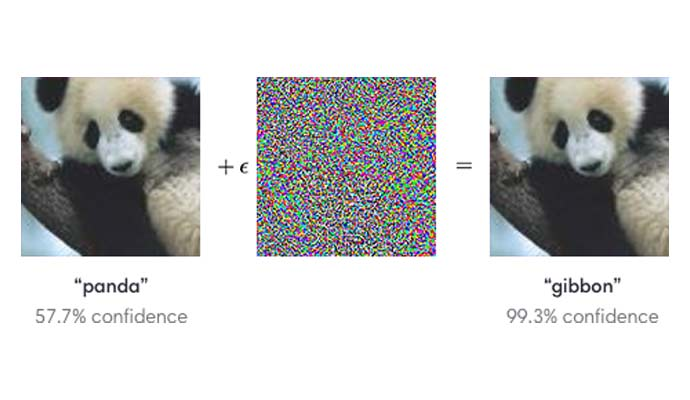
\includegraphics[width=0.5\linewidth]{Images/panda-gibbon.jpg}
  \caption{Panda misclassified to a gibbon, using carefully crafted
    noise}
  \label{fig:panda-gibbon}
\end{figure}

Countrary to one might expect, for a human eye, an adversarial example
is indistinguishable from the input that originated it. In Figure
\ref{fig:panda-gibbon} we can see that the image classified as being
the one of a gibbon is pretty identical (but they are not of course) to
the panda picture. That is why adversarial examples are a topic of
interest for researchers: they make machine learning models behave in
ways that diverge from their expected behaviour --- in ways human
\emph{fail to predict}.

In a near future where machine learning models influence real-life
decisions --- ``drive straight or stop the car?'' --- this becomes
easily dangerous\footnote{https://spectrum.ieee.org/cars-that-think/transportation/sensors/slight-street-sign-modifications-can-fool-machine-learning-algorithms}.

There are different techniques to generate these adversarial examples.
One of the most known one is called \emph{fast gradient sign} and has been
introduced by Goodfellow, et al. \cite{goodfellow6572explaining}.
There is no need to know much about this attack as many libraries
already implements this technique --- see \ref{sec:cleverhans}. In fact
we used the attack \emph{as a service} without knowing too much of the
details.
